\label{texfile:Installation}
\index{Installation}
The first step in the software installation process is to obtain the \mut\ examples, executables and database files from
\url{https://github.com/Grdbldr/MUT_Examples.git} as shown in Figure~\ref{fig:mutexamples}.  You do this by:
\begin{itemize}
     \item Clicking on the green 'Code' button.
     \item Choosing 'Download ZIP' from the drop-down menu.
\end{itemize}
Note that the ZIP file also includes the executable for \mfus.
\begin{figure}
    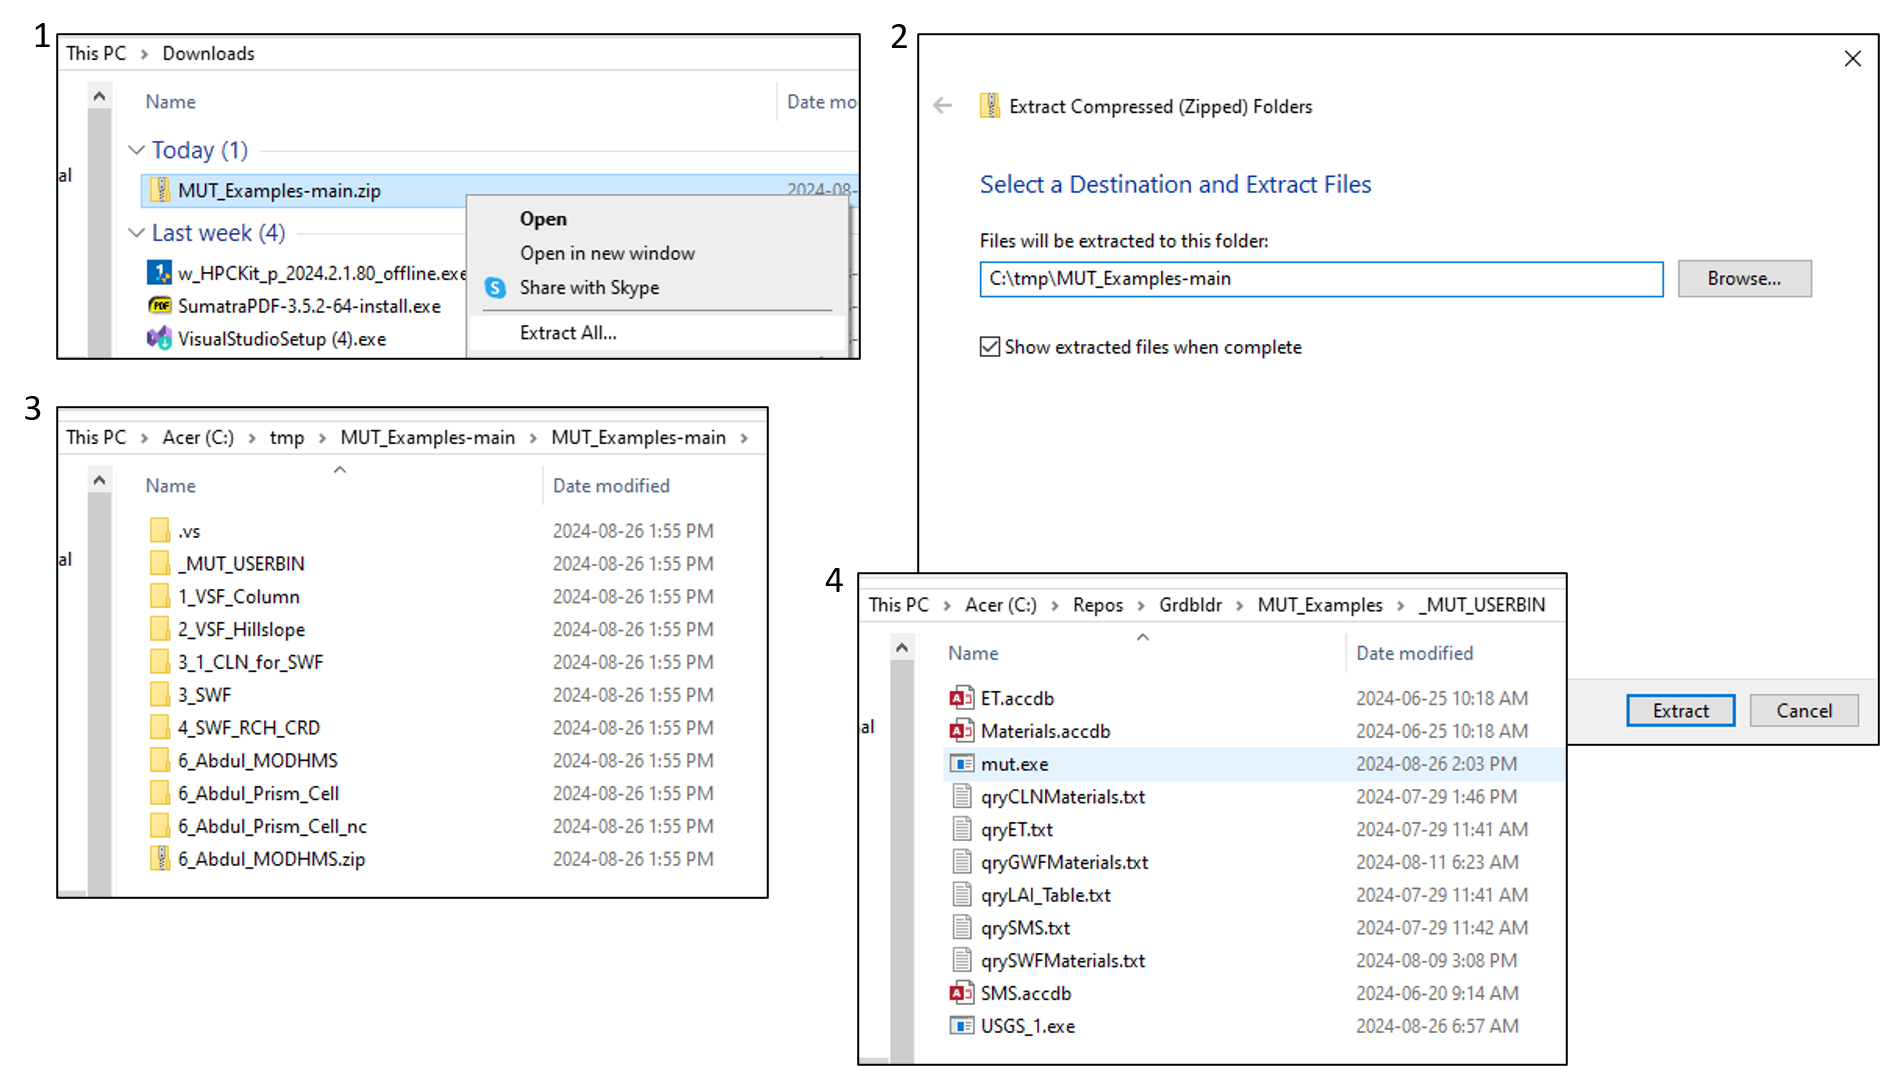
\includegraphics[width=0.95\textwidth]{DownloadMutExamples}
    \caption{Downloading the MUT\_Examples files}
    \label{fig:mutexamples}
\end{figure}

Before you run \mut\ for the first time, you need to define a windows environment variable called \bin, as shown in Figure~\ref{fig:envvar}.  You do this by:
\begin{itemize}
     \item Typing the string 'en' in the windows taskbar search field.
     \item Opening the 'Edit the system environment variables' dialogue.
     \item Clicking on the 'Environment variables...' button at the bottom of the dialogue.
     \item Adding the variable \bin.
     \item Adding the path to \bin\ to the PATH variable.
\end{itemize}
Here we have set \bin\ to be equal to \verb+c:\bin+ but you are free to choose a different drive and folder.
\begin{figure}
    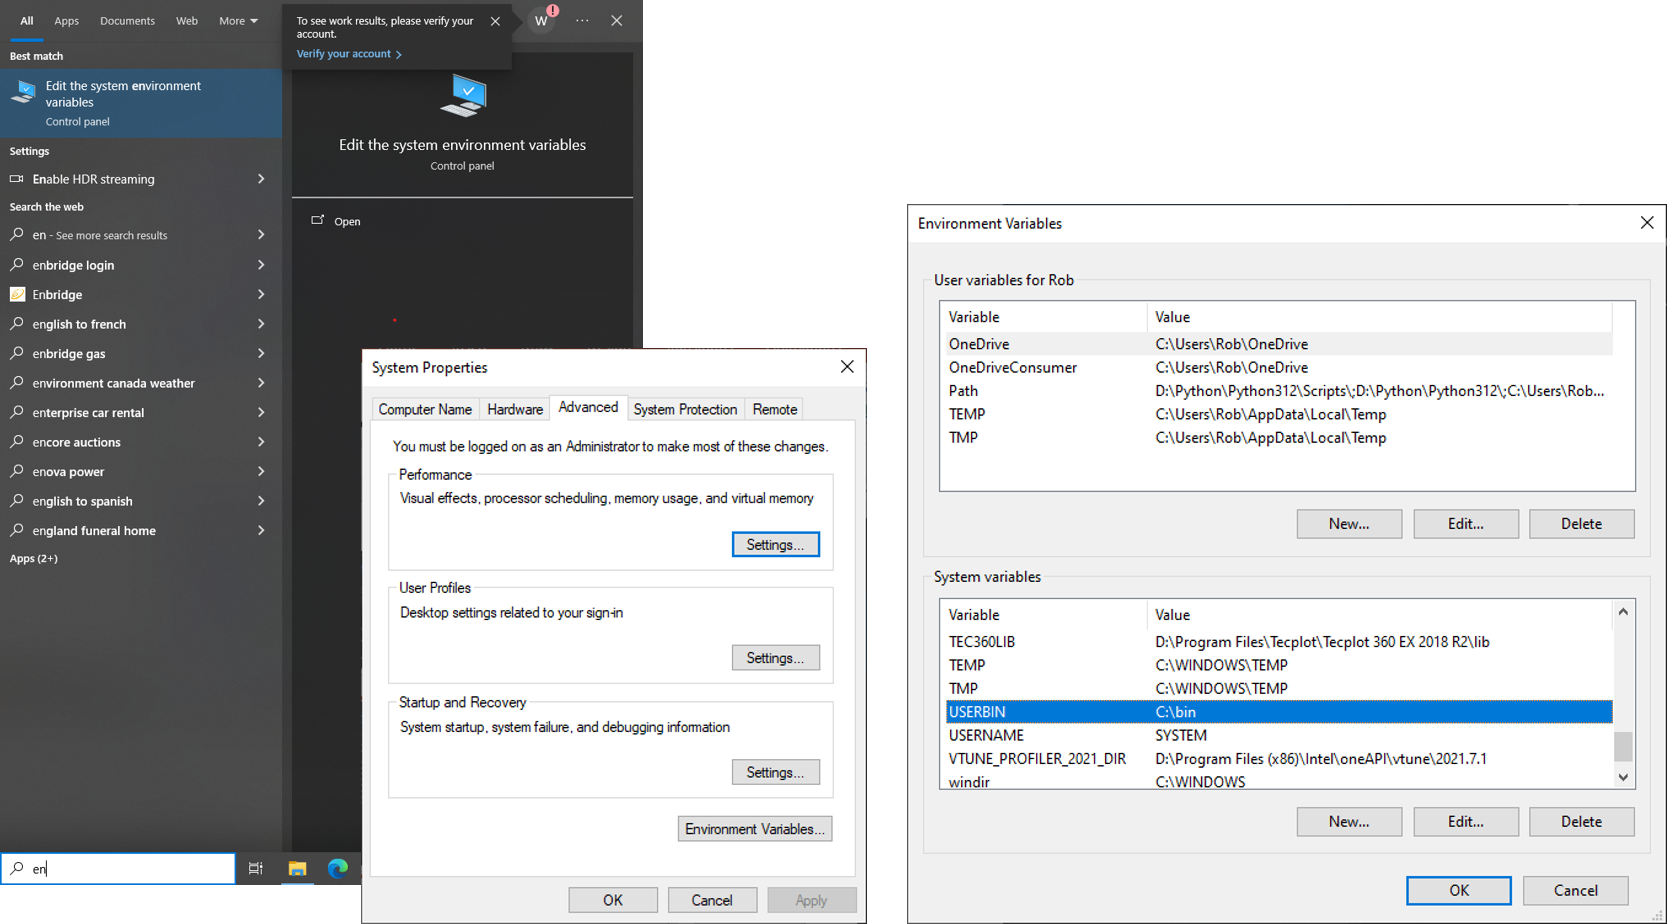
\includegraphics[width=0.95\textwidth]{EnvironmentVariables}
    \caption{Defining a new environment variable}
    \label{fig:envvar}
\end{figure}
You will need to copy the files in \verb+_MUT_USERBIN+ folder (see panel 4 in Figure~\ref{fig:mutexamples}) to the \bin\ directory.

You should now be able to run \mut\ from the command prompt.  To test this, start a new command prompt, then type \texttt{mut}, you should see the \mut\ header, shown in Figure~\ref{fig:mutheader}.  Type \texttt{CTRL C} to stop the program.
\begin{figure}
    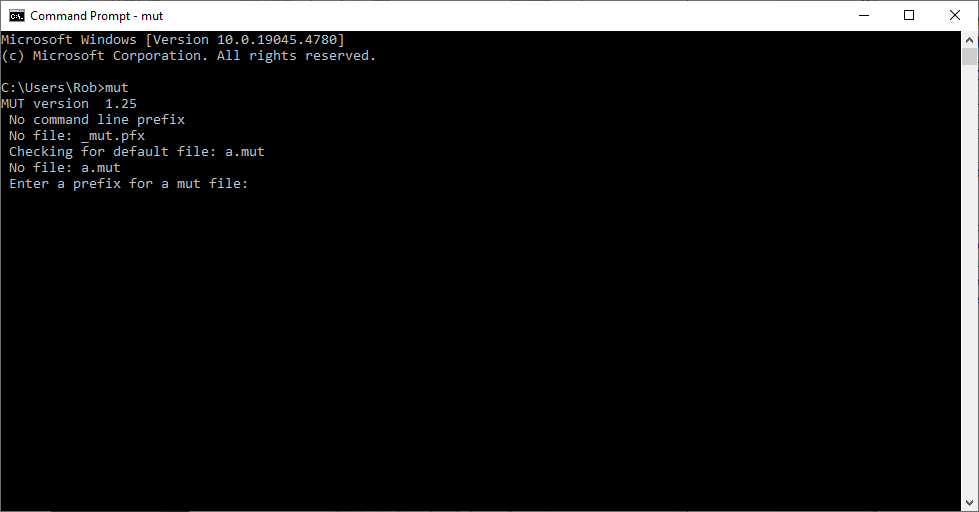
\includegraphics[width=0.95\textwidth]{mutheader}
    \caption{\mut\ Header}
    \label{fig:mutheader}
\end{figure}

You can also run \mfus\ by typing \texttt{usgs\_1}.  You should see the \mfus\ header, shown in Figure~\ref{fig:mfusheader}. Type \texttt{CTRL C} to stop the program.
\begin{figure}
    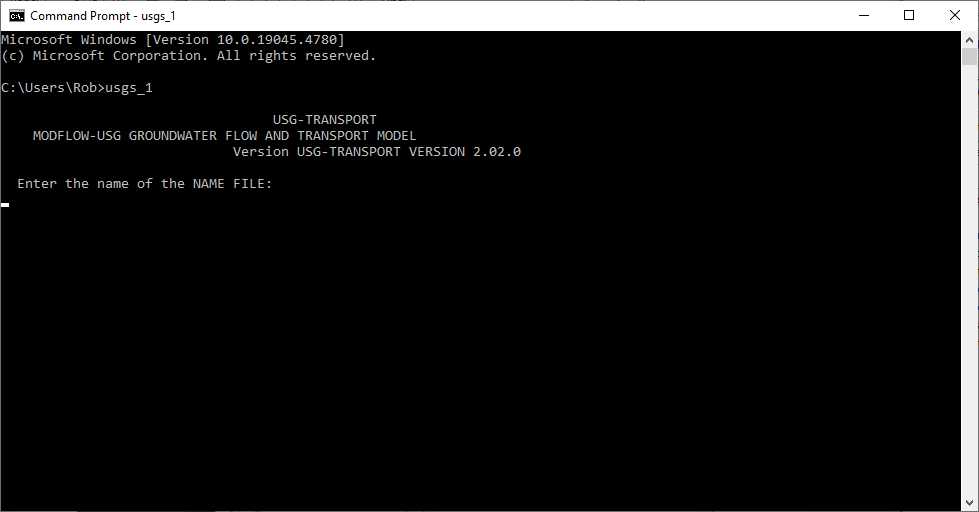
\includegraphics[width=0.95\textwidth]{mfusheader}
    \caption{\mfus\ header}
    \label{fig:mfusheader}
\end{figure}

If this is not the case, check the definitions of the \bin\ and PATH variables.  If they are correct, you may need to re-boot your computer and try again. \\

A licensed version of \tecplot\ can be obtained from \url{https://tecplot.com/products/tecplot-360/}.  They have a free 30-day trial option for those who want to assess the software before purchase.  They also offer educational discounts.

Those of you who are just interested in running the \mut\ and \mfus\ programs have completed the required  software installation tasks and can proceed to Chapter~\ref{chapter:ModelBuild}, \textbf{Model Build}. \\

Those who want to view and possibly modify and re-compile the source code for \mut\ and \mfus\ should proceed with these instructions for setting up your \windows\ programming environment.

As was stated earlier, we use and recommend \vstudio\ and \ifort. You should install \vstudio\ before \ifort, which will then be automatically integrated into \vstudio. \\

A free version of the latest \vstudio\ (currently 2022) can be obtained from \url{https://visualstudio.microsoft.com/vs/community/}. Once you are on the site just click the \texttt{Download} button.  This will download a file (e.g.\ \texttt{VisualStudioSetup.exe}) which can be run to install \vstudio.  If you already have a version of \vstudio, you can choose to keep your old version and add the latest version.  When you come to the installation options 'Workloads' page, be sure to check the option for \texttt{Desktop development with C++}, shown here:

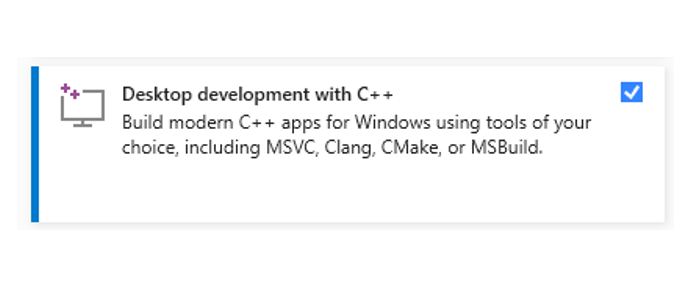
\includegraphics[width=0.6\textwidth]{vstudiooption}

A free version of the latest \ifort\ compiler can be obtained from \url{https://www.intel.com/content/www/us/en/developer/tools/oneapi/hpc-toolkit.html}.
Once you are on the site just click the \texttt{Get It Now} button to download the Intel® HPC Toolkit, which includes \ifort.  Choose the \texttt{Windows} option then the \texttt{Offline Installer} option. Now you can either fill in the required information and start the download or choose to \texttt{Continue as guest(download starts immediately)}.  This will download a file (e.g.\ \texttt{w\_HPCKit\_p\_2024.2.1.80\_offline.exe}) which can be run to install \ifort.

You can check the installion of \vstudio\ and \ifort\ by starting \vstudio\ and choosing \texttt{Create a new project}.  The window that appears should have  links for creating Fortran projects, as shown here:

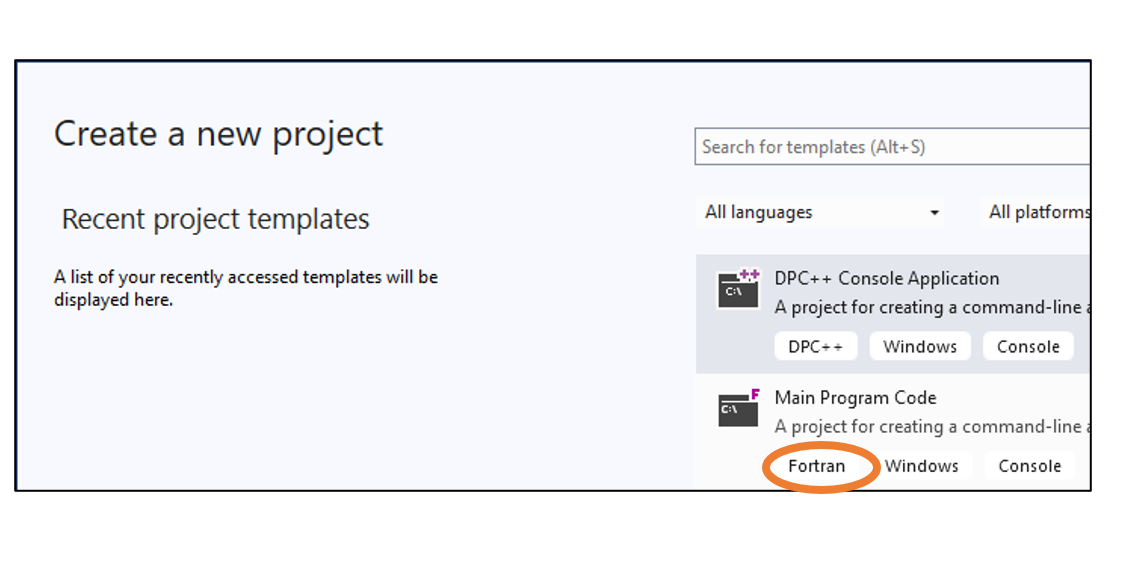
\includegraphics[width=0.8\textwidth]{createproject}

The \mut\ source files can be obtained from a \github\ repository at \url{https://github.com/Grdbldr/MUT_Source.git}.  Since \github\ has been integrated into \vstudio\, we will use it to download the \mut\ repository.  When you start \vstudio\, choose this option:

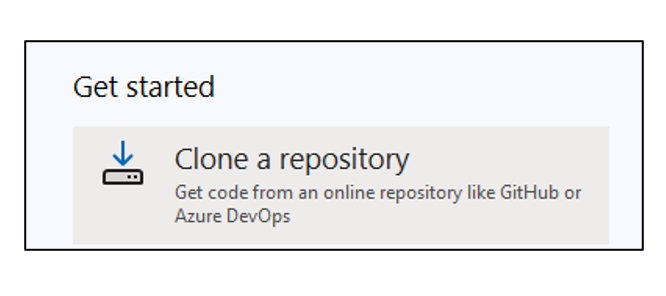
\includegraphics[width=0.4\textwidth]{clonerepo}

This opens the dialogue box shown below, where you can define the repository location on \github\ and the path to the local repository.  You can copy the link from the PDF file by right-clicking on it and choosing \texttt{Copy Link Adress}.

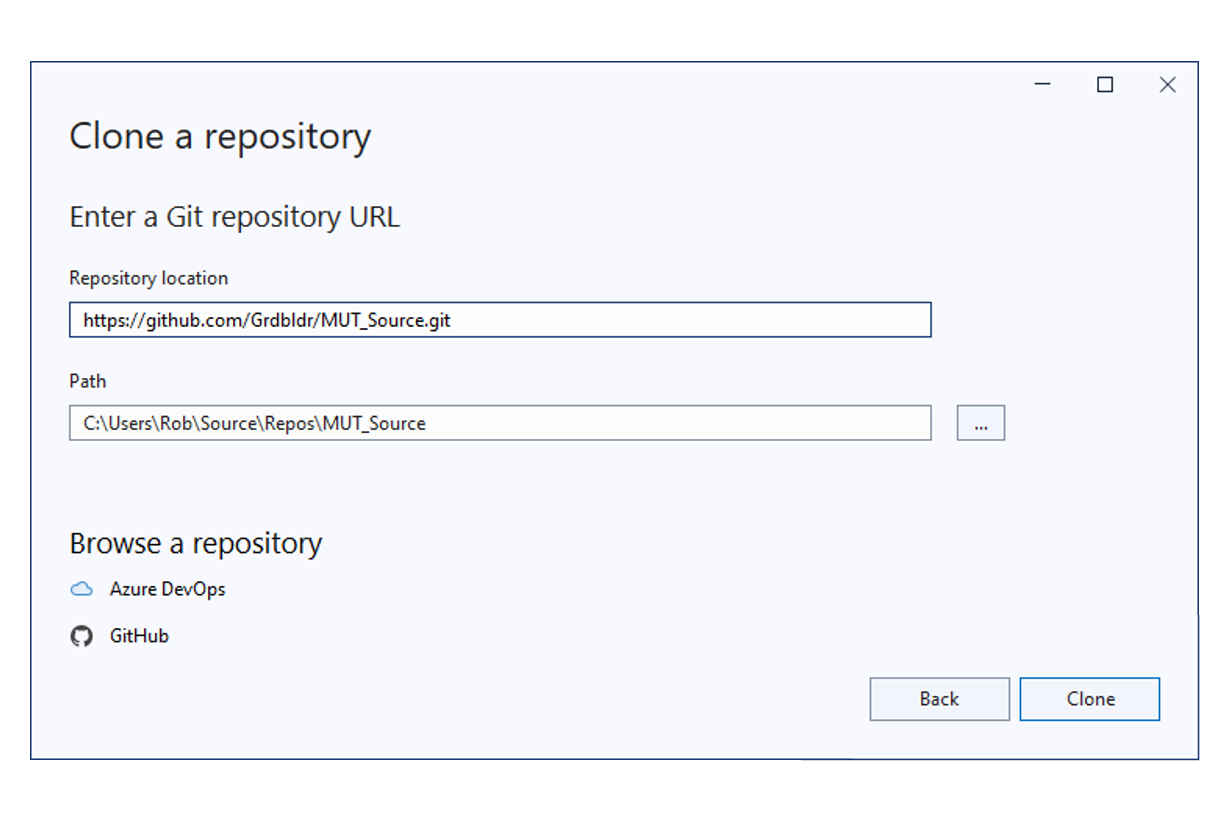
\includegraphics[width=0.7\textwidth]{clonerepodialogue}

Now choose the \texttt{GitHub} option under \texttt{Browse a Repository} and you will see this dialogue shown below, Choose \texttt{Grdbldr/MUT\_Source} from the list of repositories then click the \texttt{Clone} button.

  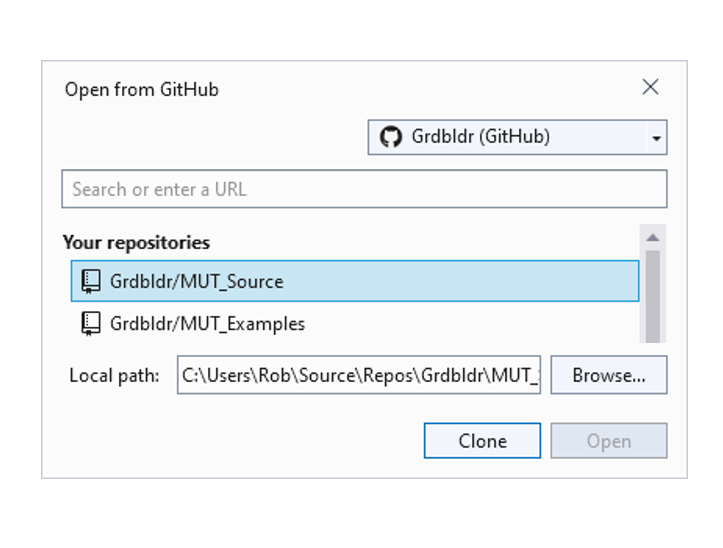
\includegraphics[width=0.45\textwidth]{clonemutsource}

Figure~\ref{fig:vstudiomutsource} shows \vstudio\ after cloning \texttt{Grdbldr/MUT\_Source}. Note the \github\ dialogue on the right side of the changes tab, with information along the bottom about the repository.  Details about using \github\ in \vstudio\ are given in Tutorial~\ref{tutorial:GitInVStudio}. \\
\begin{figure}
    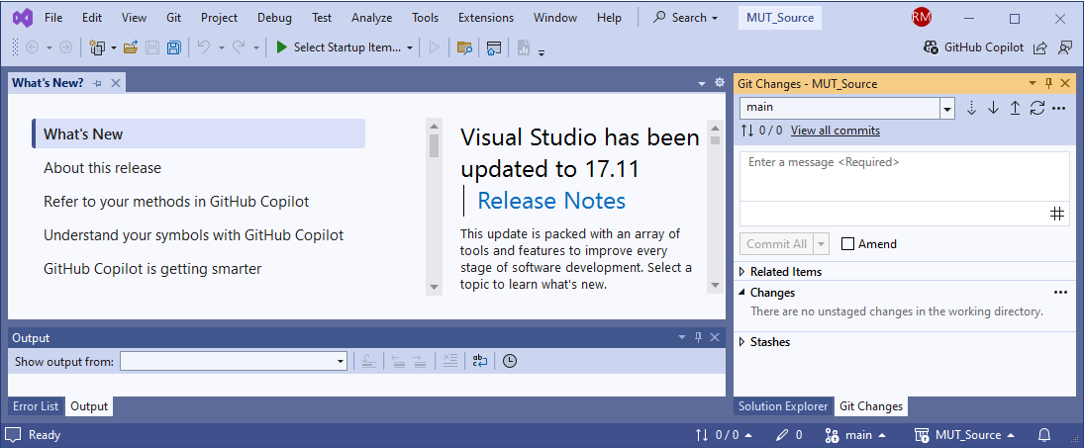
\includegraphics[width=\textwidth]{vstudiomutsource}
    \caption{\vstudio\ after cloning \texttt{Grdbldr/MUT\_Source}}
    \label{fig:vstudiomutsource}
\end{figure}

The software has been developed and tested under:
\begin{itemize}
    \item Windows 10
    \item \tecplot 360 EX 2018 R2
    \item Microsoft Visual Studio Community 2022, Version 17.11.1
    \item Intel® Fortran Compiler   2024.1
\end{itemize} 